\documentclass[12pt]{article}
\usepackage{tikz} 
\usetikzlibrary{arrows.meta} 
\usetikzlibrary{shapes,arrows}
\usetikzlibrary{matrix,calc,shapes}
\usepackage{amsmath, amssymb}




\begin{document}




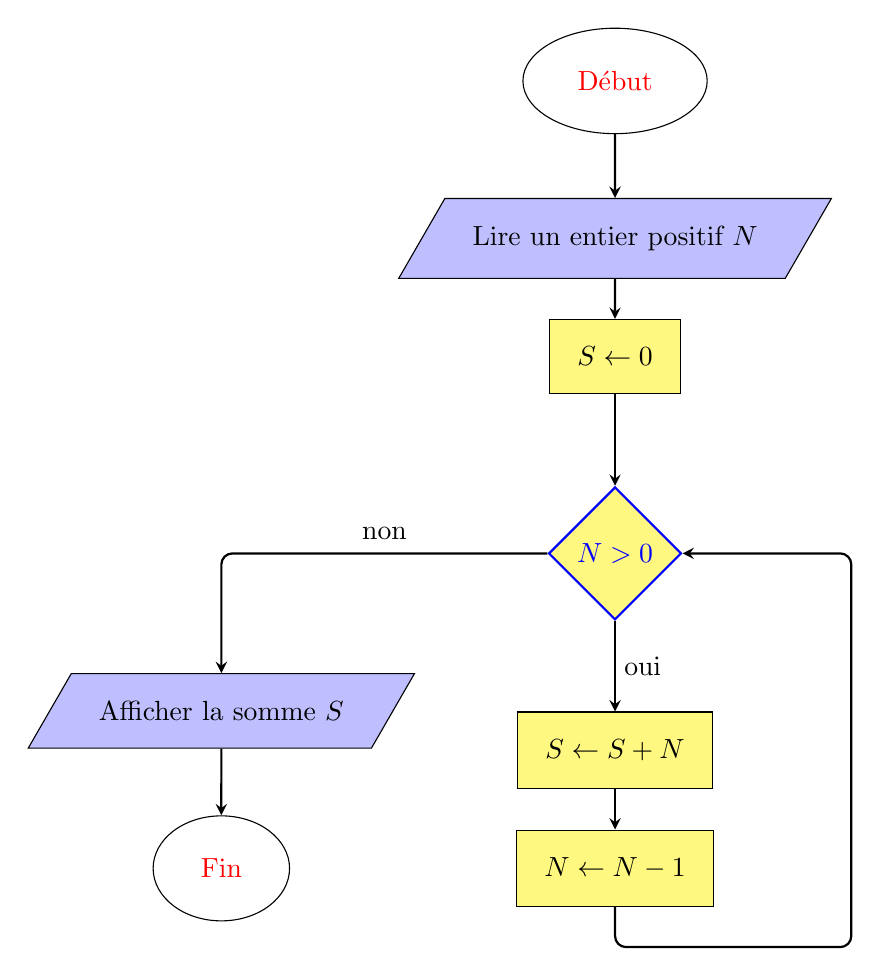
\begin{tikzpicture}
%styledesnœuds
\tikzstyle{input}=[
        draw,
        trapezium,
        trapezium left angle=60,
        trapezium right angle=120,
        inner sep=10pt,
        fill=blue!25
]
\tikzstyle{output}=[
        draw,
        trapezium,
        trapezium left angle=60,
        trapezium right angle=120,
        inner sep=10pt,
        fill=blue!25
]
\tikzstyle{debutfin}=[ellipse,draw,text=red,inner sep=10pt]
\tikzstyle{instruct}=[rectangle,draw,fill=yellow!50,inner sep=10pt]
\tikzstyle{test}=[diamond, aspect=1,thick,
draw=blue,fill=yellow!50,text=blue]
\tikzstyle{es}=[rectangle,draw,rounded corners=4pt,fill=blue!25,inner sep=10pt]
%styledesflèches
\tikzstyle{suite}=[->,>=stealth,thick,rounded corners=4pt]
%placementdesnœuds
\node[debutfin] (debut) at (0,6) {Début};
\node[input] (lire) at (0,4) {Lire un entier positif $N$};
\node[instruct] (init) at (0,2.5) {$S\leftarrow 0$};
\node[test] (test) at (0,0) {$N>0$};
\node[instruct] (plus) at (0,-2.5) {$S\leftarrow S+N$};
\node[instruct] (moins) at (0,-4) {$N\leftarrow N-1$};
\node[output] (afficher) at (-5,-2) {Afficher la somme $S$};
\node[debutfin] (fin) at (-5,-4) {Fin};
%Placementdesflèches
\draw[suite] (debut) -- (lire);
\draw[suite] (lire) -- (init);
\draw[suite] (init) -- (test.north);
\draw[suite] (test) -- (plus) node[midway,xshift=10pt]{oui};
\draw[suite] (plus) -- (moins);
\draw[suite] (moins) |- (3,-5) |- (test.east);
\draw[suite] (test) -| (afficher) node[near start,yshift=7pt]{non};
\draw[suite] (afficher) -- (fin);
\end{tikzpicture}






\newpage





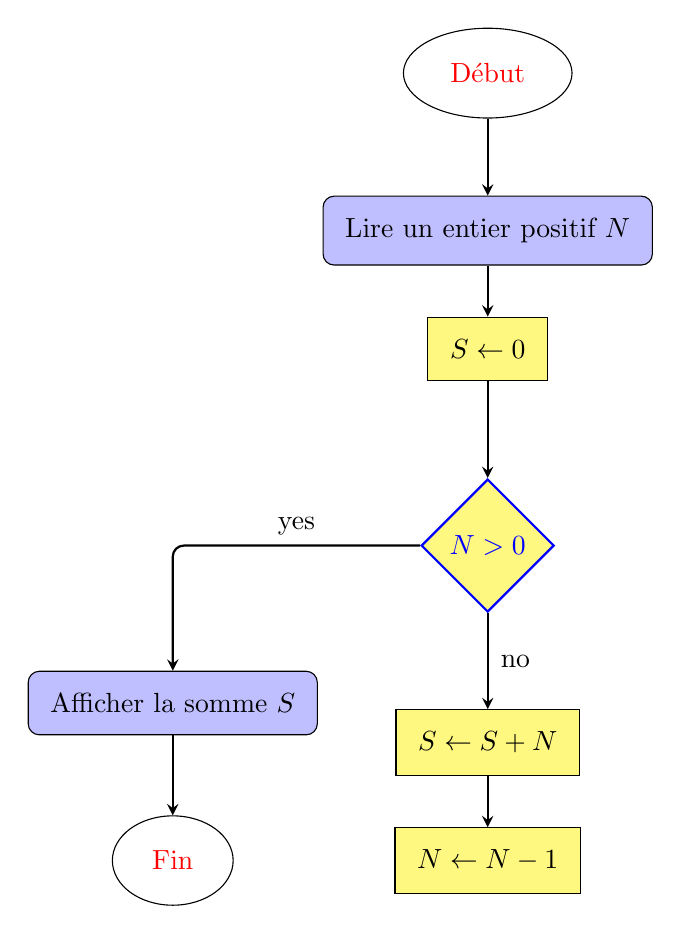
\begin{tikzpicture}
\tikzstyle{debutfin}=[ellipse,draw,text=red,inner sep=8pt]
\tikzstyle{instruct}=[rectangle,draw,fill=yellow!50,inner sep=8pt]
\tikzstyle{test}=[diamond, aspect=1,thick,
draw=blue,fill=yellow!50,text=blue]
\tikzstyle{es}=[rectangle,draw,rounded corners=4pt,fill=blue!25,inner sep=8pt]

\node[debutfin] (debut) at (0,6) {Début};
\node[es] (lire) at (0,4) {Lire un entier positif $N$};
\node[test] (test) at (0,0) {$N>0$};
\node[instruct] (init) at (0,2.5) {$S\leftarrow 0$};
\node[instruct] (plus) at (0,-2.5) {$S\leftarrow S+N$};
\node[instruct] (moins) at (0,-4) {$N\leftarrow N-1$};

\node[es] (afficher) at (-4,-2) {Afficher la somme $S$};
\node[debutfin] (fin) at (-4,-4) {Fin};

\tikzstyle{suite}=[->,>=stealth,thick,rounded corners=4pt]
\draw[suite] (debut) -- (lire);
\draw[suite] (lire) -- (init);
\draw[suite] (init) -- (test.north);
\draw[suite] (test) -- node[midway,xshift=10pt] {no} (plus);
\draw[suite] (plus) -- (moins);
\draw[suite] (test) -|  node[near start,yshift=7pt] {yes} (afficher);
\draw[suite] (afficher) -- (fin);

\end{tikzpicture}














 
\begin{tikzpicture}[node distance = 3cm, auto]
\tikzset{
startend/.style = {draw, circle},
input/.style = {draw, trapezium, trapezium left angle=70, trapezium right angle=-70, minimum height=4em},
print/.style = {draw, trapezium, trapezium left angle=-70, trapezium right angle=-70, minimum height=4em},
operation/.style = {rectangle, draw, text width=17em, text centered, minimum height=4em},
question/.style = {diamond, draw, text width=8em, text centered, inner sep=0pt},
line/.style = {draw, -latex'}
}


     \node [startend] (start) {Start};
     \node [input, below of=start] (input) {$h,n_{0},x_{0},y_{0}$};
     \node [operation, below of=input] (operationa) {$n=0$};
     \node [operation, below of=operationa] (operationb) {$n=n+1$\\ $x_{n}=x_{n-1}+h$\\ $y_{n}=y_{n-1}+hf(x_{n-1},y_{n-1})$};
     \node [question, below of=operationb] (question) {$x_{n}\geq{}x_{0}+n_{0}h$};
     \node [print, below of=question] (print) {$x_{0},y_{0}$};
     \node [startend, below of=print] (end) {End};
 
     \path [line] (start) -- (input);
     \path [line] (input) -- (operationa);
     \path [line] (operationa) -- (operationb);
     \path [line] (operationb) -- (question);
     \path [line] (question) -- node {No} (operationb);
     \path [line] (question) -- node {Yes} (print);
     \path [line] (print) -- (end);
\end{tikzpicture}




















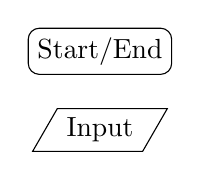
\begin{tikzpicture}
\tikzset{
    start-end/.style={
        draw,
        rectangle,
        rounded corners,
    },
    input/.style={ % requires library shapes.geometric
        draw,
        trapezium,
        trapezium left angle=60,
        trapezium right angle=120,
    },
    operation/.style={
        draw,
        rectangle
    },
    loop/.style={ % requires library shapes.misc
        draw,
        chamfered rectangle,
        chamfered rectangle xsep=2cm
    },
    decision/.style={ % requires library shapes.geometric
        draw,
        diamond,
        aspect=#1
    },
    decision/.default=1,
    print/.style={ % requires library shapes.symbols
        draw,
        tape,
        tape bend top=none
    },
    connection/.style={
        draw,
        circle,
        radius=5pt,
    },
    process rectangle outer width/.initial=0.15cm,
    predefined process/.style={
        rectangle,
        draw,
        append after command={
        \pgfextra{
          \draw
          ($(\tikzlastnode.north west)-(0,0.5\pgflinewidth)$)--
          ($(\tikzlastnode.north west)-(\pgfkeysvalueof{/tikz/process rectangle outer width},0.5\pgflinewidth)$)--
          ($(\tikzlastnode.south west)+(-\pgfkeysvalueof{/tikz/process rectangle outer width},+0.5\pgflinewidth)$)--
          ($(\tikzlastnode.south west)+(0,0.5\pgflinewidth)$);
          \draw
          ($(\tikzlastnode.north east)-(0,0.5\pgflinewidth)$)--
          ($(\tikzlastnode.north east)+(\pgfkeysvalueof{/tikz/process rectangle outer width},-0.5\pgflinewidth)$)--
          ($(\tikzlastnode.south east)+(\pgfkeysvalueof{/tikz/process rectangle outer width},0.5\pgflinewidth)$)--
          ($(\tikzlastnode.south east)+(0,0.5\pgflinewidth)$);
        }  
        },
        text width=#1,
        align=center
    },
    predefined process/.default=1.75cm,
    man op/.style={ % requires library shapes.geometric
        draw,
        trapezium,
        shape border rotate=180,
        text width=2cm,
        align=center,
    },
    extract/.style={
        draw,
        isosceles triangle,
        isosceles triangle apex angle=60,
        shape border rotate=90
    },
    merge/.style={
        draw,
        isosceles triangle,
        isosceles triangle apex angle=60,
        shape border rotate=-90
    },
}
\node[start-end] (start) {Start/End};
\node[below of=start,input](inp){Input};
\end{tikzpicture}






\end{document}